\documentclass[12pt]{article}
\usepackage{../mcm}
\graphicspath{{../images/}}

\begin{document}
\section{Shapes}

\subsection{Assumptions}
\begin{enumerate}
  \item The area is fixed to $A$. To determine the optimal shape, we use $A=1$. The effects of varying $A$ is explored separately.
  \item By the symmetry of the oven and positions of the heat sources, we may assume that an ideal shape must have the symmetry of some dihedral group. We begin with exploring shapes that have the dihedral group of order 8, $D_4$.
\end{enumerate}

\subsection{Mutation, Area-Preserving Map, and Chaos}
In GA, mutation serves as a means of introducing new kinds of shapes that are potentially successful.
Since our goal is to compare different shapes with fixed area, we need to mutate shapes in a way such that does not alter the area.
Thus, mutation of shapes naturally require \textit{area-preserving map}.
Area-preserving map is a measure-preserving map in a two-dimensional sense, i.e. $m(L^{-1}) = m(L)$, where $m$ is the Lebesgue measure.
For example, suppose $L$ is a linear transformation.
If $\det(L) = 1$ then it is an area-preserving map; the class of such maps correspond to the special linear group $SP(2,R)$.
A typical member of $SP(2,R)$, however, does not bring about a radical change to a shape.
For example, the matrix
\begin{equation*}
\begin{pmatrix}
    \cos\theta & -\sin\theta  \\
    \sin\theta & \cos\theta  
  \end{pmatrix}
\end{equation*}
as a linear map corresponds to the rotation by $\theta$. 
Although this characteristic is suitable as a way of introducing slight modifications to a pre-existing shape, applications of such maps would not create an entirely new shape.
The observation motivates us to employ chaotic maps instead.
We can think of chaotic maps as having a higher mutation rate than non-chaotic maps.
Hence, we can use chaotic maps as a way of creating a random shape, which would correspond to generating a random rational number in a usual GA.
Mutations of shapes by area-preserving chaotic maps allow our GA to explore the solution space that would not be easily accessible by non-chaotic transformations.
In particular, we employ two chaotic maps: the \textbf{cat map} and \textbf{kick map}.

\subsection{The Cat Map}
We use the cat map (commonly refered to as the "Arnold's Cat Map") to mutate shapes.
Arnold's cat map is a chaotic, area-preserving map on a two-dimensional torus \citep{hilborn}.
The cat map $F$is defined as
\begin{equation*}
  F: (x,y) \mapsto (2x + y, x + y) \mbox{ (mod 1)}.
\end{equation*}
The corresponding matrix is
\begin{equation*}
A =
\begin{pmatrix}
    2 & 1  \\
    1 & 1  
  \end{pmatrix},
\end{equation*}
and clearly, $\det(A) = 1$.
In order to obtain a wider variety of shapes, we parametrize the Arnold's map as follows:
\begin{equation*}
  F: (x,y) \mapsto (kx + (k-1)y, x + y) \mbox{ (mod 1)},
\end{equation*}
where $k \in \mathbb{R}$, $0 \leq k \leq 5$.
Note that the determinant of the corresponding matrix
\begin{equation*}
\begin{pmatrix}
    k & k-1  \\
    1 & 1  
  \end{pmatrix}
\end{equation*}
is one.
Therefore, the parametrized Arnold's map is area-preserving.
\begin{figure}[t]
  \centering
  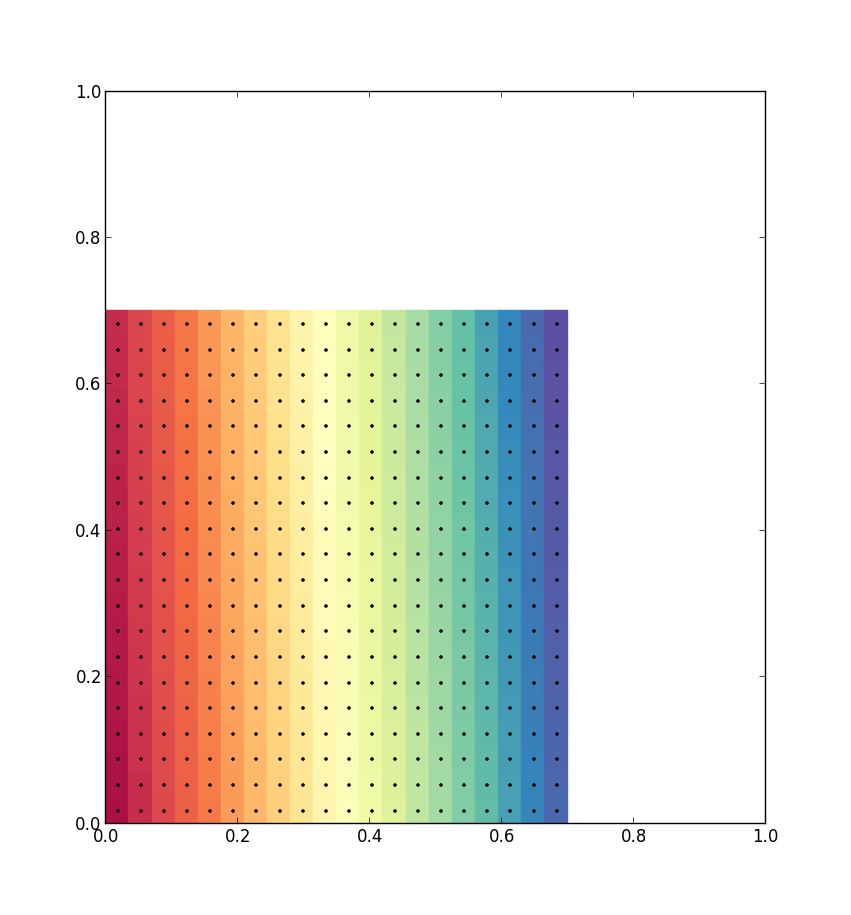
\includegraphics[width=0.6\textwidth]{square049_400}
  \caption{A square $A = 0.49$ (i.e. the length of each edge is 0.7). Each square consists of patches. This square, for instance, consists of 400 patches, each represented with different colors.}
  \label{fig:catmap_demo}
\end{figure}
The parameter $k$ determines the map's tendency to distort the square to the $x$-direction.
The closer the value of $k$ is to $0$, the more the unit square is stretched in the $x$-direction, while as $k$ gets larger, the stretching tends toward the diagonal~\ref{fig:catmap_demo}.
\begin{figure}[t]
  \centering
  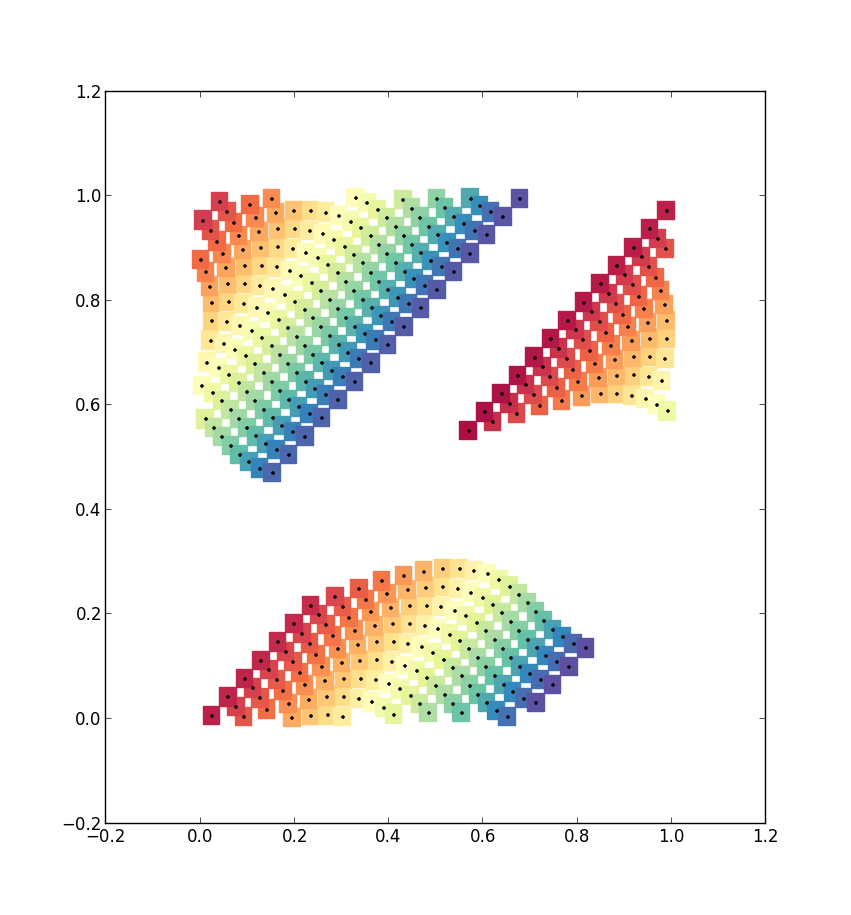
\includegraphics[width=0.4\textwidth]{catmap_05}
  \hspace{2cm}
  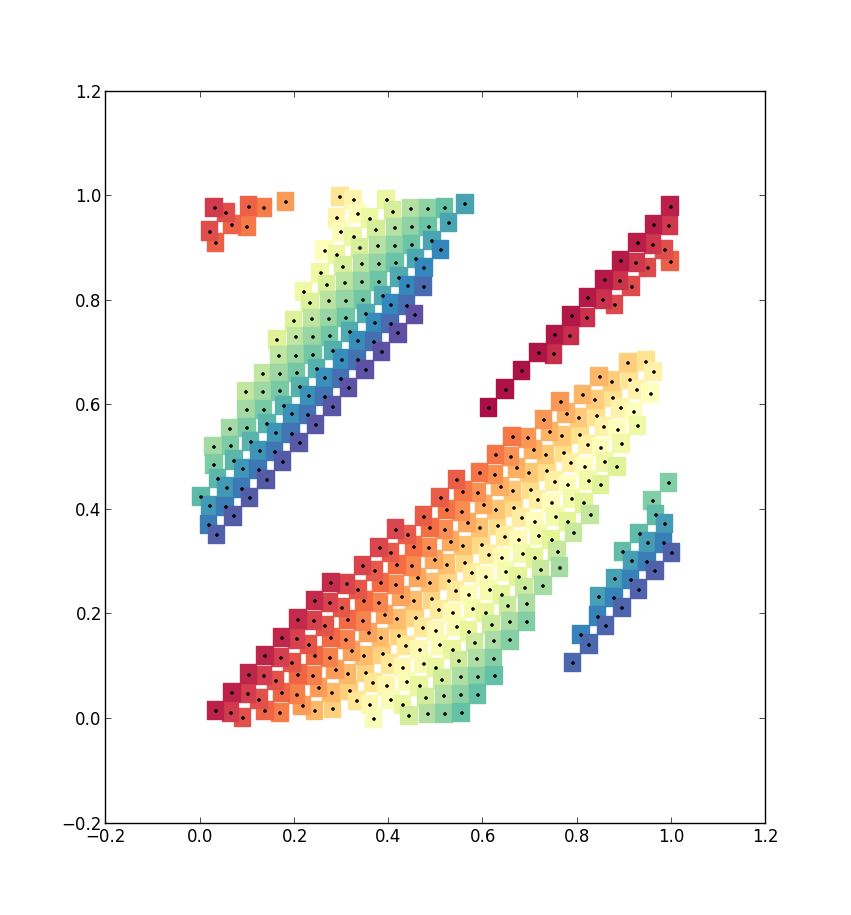
\includegraphics[width=0.4\textwidth]{catmap_3}
  \caption{Cat Map. left: $k=0.5$; right: $k = 3$. After one iteration each. The one with smaller $k$ is streched to the horizontal direction more.}
  \label{fig:catmap_demo}
\end{figure}

Although, $k$ can be any real number, $k_0$ and $k_0$ result in effectively the same transformation, since the mapped images would be symmetric about the origin, and we take modulus 1 of the points.

\subsection{The Kick Map}
The other area-preserving chaotic map that we employ, the \textit{kick map}, is usually called the Chirikov's Standard Map. \citep{ott}.
\begin{align*}
  y \mapsto y + k \sin x \mbox{ (mod $2\pi$)}
  x \mapsto x + y \mbox{ (mod $2\pi$)},
\end{align*}
where updates of $y$ and $x$ are done asyncronously ($y$ first).

\end{document}
